% Created 2025-04-10 Thu 16:41
% Intended LaTeX compiler: lualatex
\documentclass[a4paper,12pt]{article}
\usepackage{amsmath}
\usepackage{fontspec}
\usepackage{graphicx}
\usepackage{longtable}
\usepackage{wrapfig}
\usepackage{rotating}
\usepackage[normalem]{ulem}
\usepackage{capt-of}
\usepackage{hyperref}
\usepackage{fontspec}
\usepackage[french]{babel}
\usepackage[autolanguage]{numprint}
\usepackage{amsfonts,amssymb,amsmath,mathrsfs,stmaryrd}
\usepackage[default]{sourcesanspro}
\usepackage[top=2.4cm, bottom=2.4cm, left=2.16cm, right=2.16cm]{geometry}
\usepackage{setspace,fancyhdr,indentfirst,adjustbox,caption,multicol,lastpage,datetime,authblk,ifthen}
\setlength{\columnsep}{0.8cm}
\setlength{\marginparwidth}{1.6cm}
\setlength{\parindent}{0pt}
\setcounter{secnumdepth}{0}
\setcounter{page}{1}
\usepackage[toc,page]{appendix}
\usepackage{array,booktabs,multirow,tabularx,colortbl,diagbox,makecell,ltablex}
\usepackage[table]{xcolor}
\usepackage{enumitem}\setlist{nosep}\setlist[itemize]{leftmargin=*}
\usepackage{graphicx,xcolor,pgf,tikz,pgfplots,pgfplotstable}
\usepackage{algorithm2e,algorithm,arydshln,subcaption}
\usepackage{forest}
\usetikzlibrary{calc,positioning,shapes,arrows,arrows.meta,fit,automata,quotes}
\pgfplotsset{compat=1.18}
\usepackage[acronym]{glossaries}
\makenoidxglossaries
\usepackage{fvextra,csquotes}
\usepackage{etoolbox}
\definecolor{customgray}{HTML}{505050}
\usepackage{caption}
\usepackage{wrapfig}
\usepackage{listings}
\usepackage{microtype}
\usepackage[colorinlistoftodos]{todonotes}
\usepackage{orcidlink}
\usepackage{fvextra}
\usepackage{url,hyperref}
\hypersetup{colorlinks=true, linkcolor=customgray, citecolor=customgray, urlcolor=customgray, pdfborder={0 0 0}}
\author{Cyprien PIERRE \orcidlink{0009-0009-9040-6795}}
\date{2025-04-10}
\title{Exploration de l'écosystème applicatif de PostgreSQL\\\medskip
\large Note de veille technologique}
\hypersetup{
 pdfauthor={Cyprien PIERRE \orcidlink{0009-0009-9040-6795}},
 pdftitle={Exploration de l'écosystème applicatif de PostgreSQL},
 pdfkeywords={},
 pdfsubject={},
 pdfcreator={},
 pdflang={French}}
\usepackage[style=backend=biber,style=iso-numeric,doi=true,isbn=true,mincrossrefs=1,autocite=superscript]{biblatex}
\addbibresource{~/org/references.bib}
\begin{document}

\maketitle
\begin{abstract}
Abstract
\end{abstract}

\textbf{Mots clés : }\keywords{Mots clés}

\begin{multicols*}{2}
\section*{Introduction}
\label{sec:org011d216}
Contexte

\begin{figure}[H]
\centering
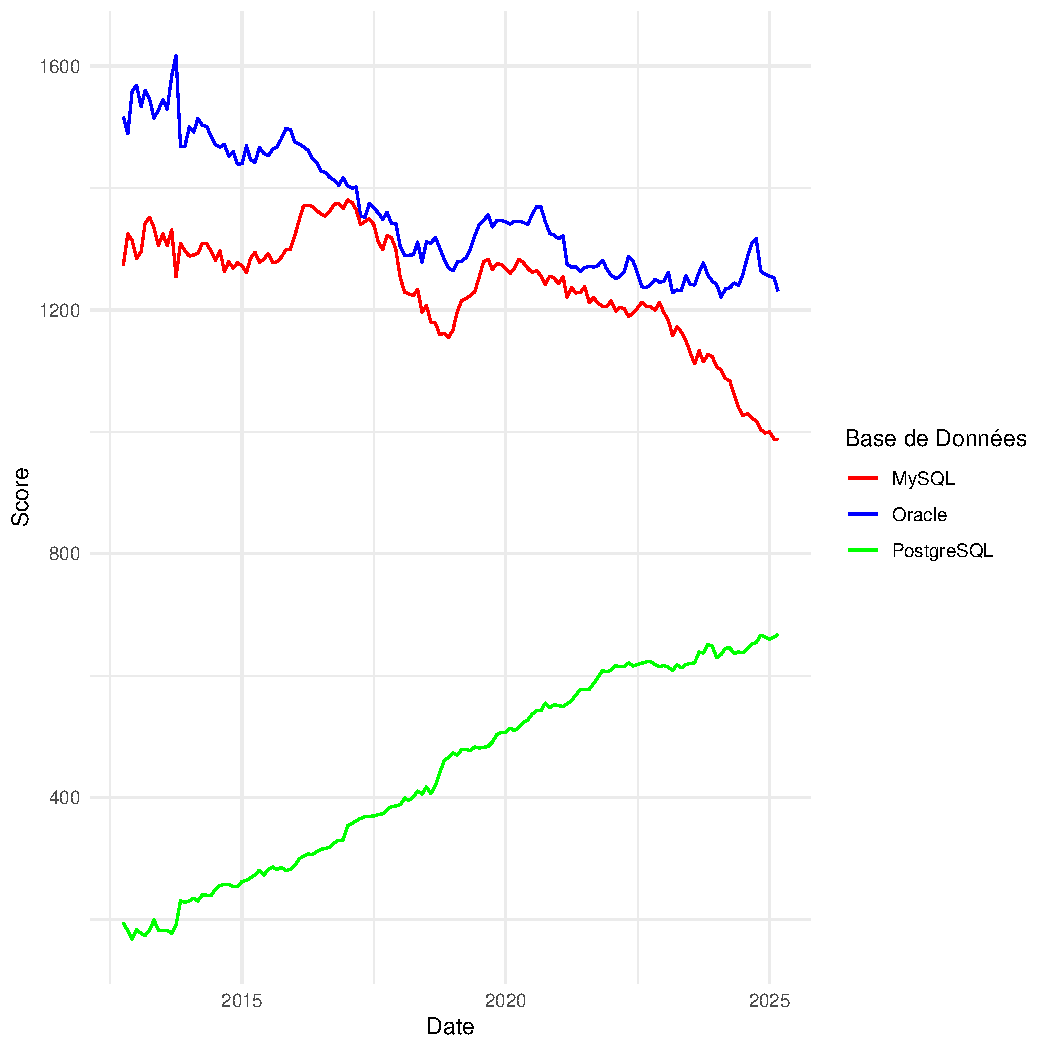
\includegraphics[width=.9\linewidth]{charts/top5.pdf}
\caption{\label{fig:orga650cb8}Tendances DB-Engine Ranking pour Oracle, MySQL, et PostgreSQL}
\end{figure} 

Objectif 

Enjeux

Méthodologie

Concentration sur les projets les plus populaires, sourcés via \href{https://gist.github.com/cpursley/c8fb81fe8a7e5df038158bdfe0f06dbb}{PostgreSQL is Enough} et \href{https://gist.github.com/joelonsql/e5aa27f8cc9bd22b8999b7de8aee9d47}{1000+ PostgreSQL Extensions}, filtré à plus de 100 étoiles et dont les développements sont toujours en cours (Mars 2025).
\section*{Fondamentaux techniques}
\label{sec:org12498be}
\subsection*{Extensions multi-modèles}
\label{sec:org6e967d1}
Bien que PostgreSQL soit initialement une base de données relationnelle orientée objet, il permet de créer des types de données personnalisés pour en étendre ses fonctionnalités.

Associé à ses capacités d'extensions, cette capacité de modification du logiciel lui permet de prendre un charge la quasi totalité des modèles de données existantes comme à venir.

Un grand nombre d'extensions communautaires, parfois portées par des entreprises, sont employés à cet effet.
\subsubsection*{Relationnel étendu}
\label{sec:org32f95a3}
\begin{description}
\item[{\href{https://github.com/tembo-io/pg\_auto\_dw}{pg\_auto\_dw}}] An auto data warehouse extension for Postgres
\item[{\href{https://github.com/darold/pgtt}{pgtt}}] extension to create, manage and use Oracle-style Global Temporary Tables and the others RDBMS.
\end{description}
\subsubsection*{Traitement en temps réel}
\label{sec:org9efd3c1}
\begin{table}[H]
\caption{Ingestion des données en temps réel}
\centering
\begin{tabular}{ll}
Nom & Particularité\\
\hline
\href{https://github.com/timescale/timescaledb}{TimescaleDB} & Hypertables\\
 & Chunking\\
 & Compression TSPC\\
\href{https://github.com/tembo-io/pg\_timeseries}{pg\_timeseries} & time-series tables\\
 & \\
 & \\
\href{https://github.com/pipelinedb/pipelinedb}{PipelineDB} & \textbf{Discontinued}\\
 & Streaming\\
 & \\
\end{tabular}
\end{table}

\begin{description}
\item[{\href{https://github.com/arkhipov/temporal\_tables}{temporal\_tables}}] Temporal Tables PostgreSQL Extension
\item[{\href{https://github.com/xocolatl/periods}{periods}}] recreates the behavior defined in SQL:2016 (originally in SQL:2011) around periods and tables with SYSTEM VERSIONING.
\end{description}

\begin{table}[H]
\caption{Execution programmée de scripts}
\centering
\begin{tabular}{ll}
Nom & Particularité\\
\hline
\href{https://github.com/cybertec-postgresql/pg\_timetable}{pg\_timetable} & Plannificateur d'évènement\\
 & \\
 & \\
\href{https://github.com/citusdata/pg\_cron}{pg\_cron} & Execution periodique\\
 & \\
 & \\
\href{https://github.com/tembo-io/pg\_later}{pg\_later} & Prééxecution\\
 & \\
 & \\
\href{https://github.com/CyberDem0n/bg\_mon}{bg\_mon} & Moniteur d'arrière plan\\
 & \\
 & \\
\end{tabular}
\end{table}

\begin{table}[H]
\caption{Capture et traitement d'évènements dans la base de données}
\centering
\begin{tabular}{ll}
Nom & Particularité\\
\hline
\href{https://github.com/eulerto/wal2json}{wal2json} & Changeset extraction\\
 & JSON output\\
 & \\
\href{https://github.com/cpursley/walex}{walex} & CDC in Elixir\\
 & \\
 & \\
\end{tabular}
\end{table}
\subsubsection*{Géospatial}
\label{sec:org9752d82}
\href{https://github.com/postgis/postgis}{PostGIS} est l'une des extensions de PostgreSQL les plus connues. Elle permet principalement de prendre en charge des modèles de données géographiques, géométriques et géospaciales.

\begin{table}[H]
\caption{Outils de manipulation de données géospaciales}
\centering
\begin{tabular}{ll}
Nom & Particularité\\
\hline
\href{https://github.com/pgRouting/pgrouting}{pgRouting} & Routage géospacial\\
 & Analyse de réseau\\
 & \\
\href{https://github.com/MobilityDB/MobilityDB}{MobilityDB} & Analyse et de gestion\\
 & des trajectoires\\
 & \\
 & \\
\href{https://github.com/zachasme/h3-pg}{h3-pg} & bindings for Uber's H3\\
 & \\
 & \\
\href{https://github.com/pgpointcloud/pointcloud}{pgpointcloud} & Storing LIDAR data\\
 & \\
 & \\
\href{https://github.com/Giswater/giswater\_dbmodel}{giswater\_dbmodel} & SQL files for\\
 & Giswater's\\
 & database model\\
\end{tabular}
\end{table}


\begin{figure}[H]
\centering

\includegraphics[height=1.2cm]{icons/pg-geospacial.pdf}
\caption{\label{fig:orgbcf62c9}Logos : PostGIS, pgRouting, MobilityDB, H3, GISWater}
\end{figure}

\begin{description}
\item[{\href{https://github.com/dr-jts/pg\_svg}{pg\_svg}}] Postgres/PostGIS functions for generating SVG documents
usage : génération de cartes, de plans, etc.
\item Raster format, Bitmap extensions etc.
\end{description}
\subsubsection*{Données non structurées}
\label{sec:org334dcd8}
\begin{description}
\item[{\href{https://github.com/apache/age}{Apache AGE}}] Graph database optimized for fast analysis and real-time data processing. It is provided as an extension to PostgreSQL (OpenCypher)
\end{description}

\begin{description}
\item[{\href{https://github.com/microsoft/documentdb}{MS DocumentDB}}] offers a native implementation of document-oriented NoSQL database, enabling seamless CRUD operations on BSON data types within a PostgreSQL framework
\item[{\href{https://github.com/JasperFx/marten}{Marten}}] .NET Transactional Document DB and Event Store on PostgreSQL
\end{description}

\begin{figure}[H]
\centering

\includegraphics[height=1.2cm]{icons/pg-documents.pdf}
\caption{\label{fig:orgfda4b73}Logos : Apache AGE, FerretDB, pg\_duck, Marten, Pongo}
\end{figure}

\begin{description}
\item[{\href{https://github.com/postgrespro/jsquery}{JsQuery}}] json query language with GIN indexing support
\item[{\href{https://github.com/FerretDB/FerretDB}{FerretDB}}] A proxy that converts MongoDB 5.0+ wire protocol queries to SQL and uses PostgreSQL with DocumentDB extension as a database engine
\item[{\href{https://github.com/robconery/dox}{dox}}] A Document Database API extension for Postgres
\end{description}

Expliquer le principe "NoSQL" et les divergences d'interprétations
\begin{description}
\item[{\href{https://github.com/supabase/pg\_graphql}{pg\_render}}] Render HTML in SQL. PostgreSQL extension
\item[{\href{https://github.com/Florents-Tselai/pgpdf}{pgpdf}}] pdf type for Postgres
\item[{\href{https://github.com/event-driven-io/Pongo}{Pongo}}] Mongo but on Postgres and with strong consistency benefits
\end{description}

Pour la mise en cache 
Solutions : pg\_catcache (LRU), pgmemcache (intégration Memcached)
Mise en cache et file d’attente : postgres’s Unlogged table puis memcache (ou equivalent)
\begin{description}
\item[{\href{https://github.com/supabase/pg\_jsonschema}{pg\_jsonschema}}] PostgreSQL extension providing JSON Schema validation

\item[{\href{https://github.com/duckdb/pg\_duckdb}{pg\_duckdb}}] a Postgres extension that embeds DuckDB's columnar-vectorized analytics engine and features into Postgres
\end{description}
\subsubsection*{Récupération d'information et IA}
\label{sec:orgb01d90a}
\begin{quote}
\emph{Dans un monde plus ouvert qu’il n’a jamais été, notre Société traverse une nouvelle mutation en passant de l’économie industrielle à l’économie du service et de la connaissance.} -- Urban-Galindo\autocite{jean-jacquesurban-galindoGestionConfigurationIngenierie2008}
\end{quote}

La mise en place d’un environnement d’apprentissage, d’exploration et de partage de connaissance offre la capacité de développer son expertise. \autocite{vidicKnowledgeAssetCompetitive2022} Il s’agit d’une opportunité stratégique de long terme permettant le maintien des connaissances au sein d’une entreprise dans un contexte de raréfaction des ressources humaines,\autocite{thoumsinQuellesStrategiesFautil2019} lutant ainsi contre l’amnésie organisationnelle.\autocite{lucierivardCycleRetentionConnaissances2010}

Discuter de l’avantage stratégique de pgvector face à des bases dédiées (Elasticsearch).

\begin{description}
\item[{\href{https://github.com/pgvector/pgvector}{pgVector}}] Implémentation des vecteurs
\item[{\href{https://github.com/timescale/pgvectorscale}{pgvectorescale}}] A complement to pgvector for high performance, cost efficient vector search on large workloads. (timescaledb)
\item[{\href{https://github.com/tembo-io/pg\_vectorize}{pg\_vectorize}}] A Postgres extension that automates the transformation and orchestration of text to embeddings and provides hooks into the most popular LLMs. This allows you to do vector search and build LLM applications on existing data with as little as two function calls.
\item[{\href{https://github.com/lanterndata/lantern}{lantern}}] PostgreSQL vector database extension for building AI applications
\end{description}

\begin{figure}[H]
\centering

\includegraphics[height=1.2cm]{icons/pg-search.pdf}
\caption{\label{fig:orgcebf87c}Logos : ParadeDB, ZomboDB, PGroonga, PostgresML, Lantern}
\end{figure}


Dans le paysage en évolution de l'IA, la malléabilité de PostgreSQL devient un avantage stratégique. Le framework PostgresML, intégrant des modules tels que pgCat, pgVector  et pg\_partman, permet d’architecturer directement au niveau de la base de données des systèmes de Machine Learning. 

\begin{description}
\item[{\href{https://github.com/postgresml/postgresml}{PostgresML}}] Postgres with GPUs for ML/AI apps
\item[{\href{https://github.com/timescale/pgai}{pgai}}] A suite of tools to develop RAG, semantic search, and other AI applications more easily with PostgreSQL (TimescaleDB)
\end{description}
Cas concret : Chatbot RAG avec pgvector + Llama2
\begin{description}
\item[{\href{https://github.com/tensorchord/pgvecto.rs}{pgvecto.rs}}] Scalable, Low-latency and Hybrid-enabled Vector Search in Postgres. Revolutionize Vector Search, not Database
\item[{\href{https://github.com/ElKornacio/pg\_auto\_embeddings}{pg\_auto\_embeddings}}] Text embeddings calculation for Postgres, without extensions. Simple, atomic, supports OpenAI/Anthropic models. Does not require any additional extensions, making it suitable for managed databases and other restricted environments
\end{description}

Korvus, Ollama\ldots{}

\begin{description}
\item[{\href{https://github.com/apache/datasketches-postgresql}{datasketches-postgresql}}] extension providing approximate algorithms based on Apache Datasketches-cpp
\item[{\href{https://github.com/cybertec-postgresql/pgfaceting}{pgfaceting}}] extension to quickly calculate facet counts using inverted index built with roaring bitmaps
\item[{\href{https://github.com/citusdata/postgresql-topn}{TopN}}] Extension that returns the top values in a database according to some criteria
\item[{\href{https://github.com/OneSparse/OneSparse}{OneSparse}}] Accelerated Sparse Linear Algebra with Postgres and SuiteSparse

\item[{\href{https://github.com/apache/arrow-flight-sql-postgresql/}{ParadeDB}}] (recherche sémantique)
\item[{\href{https://github.com/zombodb/zombodb}{ZomboDB}}] Making Postgres and Elasticsearch work together
\item[{\href{https://github.com/amutu/zhparser}{zhparser}}] zhparser is a PostgreSQL extension for full-text search of Chinese language
\item[{\href{https://github.com/pgroonga/pgroonga}{pgroonga}}] extension to use Groonga as index. PGroonga makes PostgreSQL fast full text search platform for all languages!
\item[{\href{https://github.com/pgbigm/pg\_bigm}{pg\_bigm}}] The pg\_bigm module provides full text search capability in PostgreSQL. This module allows a user to create 2-gram (bigram) index for faster full text search.
\item[{\href{https://github.com/jirutka/smlar}{smlar}}] Extension for an effective similarity search
\item[{\href{https://github.com/ChenHuajun/pg\_roaringbitmap}{pg\_roaringbitmap}}] Roaring bitmaps are compressed bitmaps which tend to outperform conventional compressed bitmaps such as WAH, EWAH or Concise. In some instances, roaring bitmaps can be hundreds of times faster and they often offer significantly better compression. They can even be faster than uncompressed bitmaps
\end{description}
\subsection*{Solutions d'optimisation}
\label{sec:org0af4708}
\begin{itemize}
\item Fonctions natives
\item Cas d'usage : Transactions ACID à haute charge (ERP, systèmes financiers)
\end{itemize}

OLTP historiquement "lent" comparé à OLAP  

\begin{description}
\item[{\href{https://github.com/postgrespro/aqo}{Aqo}}] Adaptive query optimization for PostgreSQL
\item[{\href{https://github.com/dalibo/emaj}{E-Maj}}] extension that tracks updates on tables sets with rollback capabilities
\end{description}

\begin{description}
\item[{\href{https://github.com/pgpartman/pg\_partman}{pg\_partman}}] Partition management extension for PostgreSQL
\item[{\href{https://github.com/postgrespro/pg\_pathman}{pg\_pathman}}] Partitioning tool for PostgreSQL
\item[{\href{https://github.com/ankane/pgslice}{pgslice}}] Postgres partitioning as easy as pie
\end{description}

Citus ajoute la capacité de mise à l’échelle horizontale par répartition de la charge de calcul sur les serveurs disponibles. Cette approche est appellée \texttt{sharding}. Cette extension ajoute notamment la prise en charge des tables distribuées, des tables de références, du stockage en colonnes (Wide column store) et intègre un moteur de requête distribué.

TimescaleDB propose une approche différente appelée \texttt{chunking}.

\begin{description}
\item[{\href{https://github.com/heterodb/pg-strom}{PG-Strom}}] Extension conçue pour accélérer les charges de travails en lots et les traitements analytiques en les exécutant lorsque nécessaire sur les GPU disponibles. (from HeteroDB)
\item[{\href{https://github.com/le0pard/pgtune?tab=readme-ov-file}{pgtune}}] tuning PostgreSQL config by your hardware
\end{description}
\subsubsection*{Stratégies de stockage}
\label{sec:org006e8d8}
\begin{description}
\item[{zheap}] (réduction WAL) Extension initialement créée par EDB puis maintenu par Cybertec avant d'être intégré à PostgreSQL core en version \autocite{ZheapPostgreSQLWiki2021}
\item[{pg\_dump}] (algo GZip/LZ4/Zstd)
\end{description}
How did TimescaleDB comp is working ?

Alternatives to CLUSTER and VACUUM
\begin{description}
\item[{\href{https://github.com/cybertec-postgresql/pg\_squeeze}{pg\_squeeze}}] Optimise la mémoire en réorganisant les tables et indexes en minimisant les verrouillages de la base de donnéees (Logical decoding on server only using background workers)
\item[{\href{https://github.com/reorg/pg\_repack}{pg\_repack}}] Optimise la mémoire en réorganisant les tables et indexes en minimisant les verrouillages de la base de donnéees (Triggers on Client + Server)

\item[{\href{https://github.com/CrunchyData/pg\_parquet}{pg\_parquet}}] Copy to/from Parquet in S3 or Azure Blob Storage from within PostgreSQL
\item[{\href{https://github.com/tembo-io/pg\_tier}{pg\_tier}}] Postgres Extension written in Rust, to enable data tiering to AWS S3
\item[{\href{https://github.com/scottpersinger/pgwarehouse}{pgwarehouse}}] Easily sync your Postgres database to a Snowflake, ClickHouse, or DuckDB warehouse
\item[{\href{https://github.com/supabase/storage}{storage}}] S3 compatible object storage service that stores metadata in Postgres

\item[{\href{https://github.com/crunchydata/pg\_incremental}{pg\_incremental}}] Incremental Data Processing in PostgreSQL
\item[{\href{https://github.com/sraoss/pg\_ivm}{pg\_ivm}}] Incremental View Maintenance implementation as a PostgreSQL extension
\item[{\href{https://github.com/adriangb/pgpq}{pgpq}}] Stream Apache Arrow RecordBatches into Postgres
\item[{\href{https://github.com/postgrespro/vops}{VOPS}}] VOPS provides set of standard operators for tile types, allowing to write SQL queries in the way similar with normal SQL queries.
\item[{\href{https://github.com/ankane/pgsync}{pgsync}}] Sync data from one Postgres database to another
\end{description}

\begin{description}
\item[{\href{https://github.com/orioledb/orioledb}{OrioleDB}}] Remplace le moteur de stockage dans le heap de PostgreSQL, change de row à column based querying, améliore la compression des données, nettoie automatiquement les espacces libres.
\item[{Citus}] (Microsoft) : Ajoute la capacité de mise à l’échelle horizontale par répartition de la charge de calcul sur les serveurs disponibles. Cette extension ajoute notamment la prise en charge des tables distribuées, des tables de références, du stockage en colonnes (Wide column store) et intègre un moteur de requête distribué.
\item[{\href{https://github.com/hydradatabase/columnar}{columnar}}] Postgres-native columnar storage extension
\end{description}
\subsubsection*{Indexation avancée}
\label{sec:org06914b8}
\begin{description}
\item[{BRIN}] (Big Data),
\item[{GIN}] (full-text),
\item[{Bloom}] (requêtes complexes)
\item[{\href{https://github.com/ankane/dexter}{dexter}}] Automatic indexer for Postgres
\item[{\href{https://github.com/postgrespro/rum}{RUM}}] RUM access method - inverted index with additional information in posting lists
\item[{\href{https://github.com/HypoPG/hypopg}{HypoPG}}] Création d'index hypothétique
\end{description}

\begin{quote}
\emph{An hypothetical, or virtual, index is an index that doesn't really exists, and thus doesn't cost CPU, disk or any resource to create.}
\emph{They're useful to know if specific indexes can increase performance for problematic queries, since you can know if PostgreSQL will use these indexes or not without having to spend resources to create them.} -- HypoPG
\end{quote}

\begin{description}
\item[{\href{https://github.com/supabase/index\_advisor}{index\_advisor}}] Outils pour recommander des index appropriés
\item[{\href{https://github.com/ossc-db/pg\_hint\_plan}{pg\_hint\_plan}}] Extension adding support for optimizer hints in PostgreSQL
\item[{\href{https://github.com/ossc-db/pg\_plan\_advsr}{pg\_plan\_advsr}}] extension for automated execution plan tuning
\end{description}
\subsection*{Architectures distribuées}
\label{sec:orgf2de65d}
\begin{description}
\item[{ElectricSQL}] (CRDTs)
\item[{\href{https://github.com/electric-sql/pglite}{PGLite}}] Embeddable Postgres with real-time, reactive bindings. (Wasm/Deno)
\end{description}
Use case : Synchronisation offline-first (apps mobiles)

Expliquer les intérêts en matière de performance et de fort découplage des environnements serveurs et clients.

Étudier les garanties de pglogical en environnement distribué

\begin{description}
\item[{\href{https://github.com/supabase/pg\_replicate}{pg\_replicate}}] a Rust crate to quickly build replication solutions for Postgres.
\item[{\href{https://github.com/PeerDB-io/peerdb}{peerdb}}] Fast, Simple and a cost effective tool to replicate data from Postgres to Data Warehouses, Queues and Storage
\item[{\href{https://github.com/EnterpriseDB/pg\_failover\_slots}{pg\_failover\_slots}}] PG Failover Slots is for anyone with Logical Replication Slots on Postgres databases that are also part of a Physical Streaming Replication architecture.
\item[{\href{https://github.com/2ndQuadrant/pglogical}{pglogical}}] provides logical streaming replication for PostgreSQL, using a publish/subscribe model
\item[{\href{https://github.com/EnterpriseDB/repmgr}{repmgr}}] A lightweight replication manager for PostgreSQL
\end{description}
\section*{Écosystème applicatif}
\label{sec:orgb22f6e7}
\subsection*{Compatibilité}
\label{sec:org06c5502}
\begin{quote}
\textbf{Compatibilité}, n.f.
\emph{Le fait pour un matériel ou un logiciel d'être utilisable en connexion avec d'autres matériels, d'autres logiciels, dans un système informatique défini, sans en altérer les conditions de fonctionnement.} -- CNRTL
\end{quote}

La compatibilité diffère de l'intéropérabilité par l'absence de nécessité de connaitre l'architecture interne des solutions informatiques avec lesquelles le système étudier s'interface.

\begin{description}
\item[{\href{https://github.com/supabase/pg\_net}{pg\_net}}] A PostgreSQL extension that enables asynchronous (non-blocking) HTTP/HTTPS requests with SQL
\item[{\href{https://github.com/pramsey/pgsql-http}{pgsql-http}}] Client HTTP permettant de récupérer des pages Web depuis la base de données
\end{description}

API REST :
\begin{description}
\item[{\href{https://github.com/prest/prest}{prest}}] PostgreSQL, REST, low-code, simplify and accelerate development, instant, realtime, high-performance on any Postgres application, existing or new
\item[{\href{https://github.com/PostgREST/postgrest}{PostgREST}}] API RESTful gérée par PostgreSQL
\item[{\href{https://github.com/supabase/postgres-meta}{postgres-meta}}] A RESTful API for managing your Postgres. Fetch tables, add roles, and run queries
\end{description}

API GraphQL :
\begin{description}
\item[{\href{https://github.com/graphile/crystal/tree/main/postgraphile/postgraphile}{PostGraphile}}] API GraphQL bidirectionnelle gérée par PostgreSQL I/O
\item[{\href{https://github.com/supabase/pg\_graphql}{pg\_graphql}}] Permet de requéter PostgreSQL avec une API GraphQL
\item[{\href{https://github.com/hasura/graphql-engine}{graphql-engine}}] Blazing fast, instant realtime GraphQL APIs on all your data with fine grained access control, also trigger webhooks on database events
\end{description}

WebHook :  
\begin{description}
\item[{\href{https://github.com/xataio/pgstream}{pgstream}}] Change Data Capture CLI et librairie pour PostgreSQL avec un envois via WebHook
\end{description}

WebSocket :
\begin{description}
\item[{\href{https://github.com/diogob/postgres-websockets}{postgres-websockets}}] Middleware permettant d'ajouter la prise en charge de Websockets à PostgreSQL en l'interfaçant avec les commandes LISTEN/NOTIFY
\end{description}
\subsection*{Interopérabilité}
\label{sec:org048b437}
\begin{quote}
\textbf{Interopérabilité}, n.f.
\emph{Capacité que possède un produit ou un système, dont les interfaces sont intégralement connues, à fonctionner avec d’autres produits ou systèmes existants ou futurs et ce sans restriction d’accès ou de mise en œuvre.} -- Wikitionnaire
\end{quote}

Évaluer les performances des FDW (ex. mysql\_fdw vs oracle\_fdw) et leur utilité dans les architectures hybrides.

postgres\_fdw
\begin{description}
\item[{\href{https://github.com/supabase/wrappers}{wrappers}}] Postgres Foreign Data Wrapper development framework in Rust.
\item[{\href{https://github.com/pgsql-io/multicorn2}{multicorn2}}] 
\end{description}

How it works ??
\begin{description}
\item[{\href{https://github.com/alitrack/duckdb\_fdw}{duckdb\_fdw}}] Permet de requéter DuckDB
\item[{\href{https://github.com/EnterpriseDB/hdfs\_fdw}{hdfs\_fdw}}] Permet de requéter Apache Hadoop
\item[{\href{https://github.com/EnterpriseDB/mongo\_fdw}{mongo\_fdw}}] Permet de requéter MongoDB
\item[{\href{https://github.com/EnterpriseDB/mysql\_fdw}{mysql\_fdw}}] Permet de requéter MySQL
\item[{\href{https://github.com/laurenz/oracle\_fdw}{oracle\_fdw}}] Permet de requéter Oracle
\item[{\href{https://github.com/adjust/parquet\_fdw}{parquet\_fdw}}] Permet de requéter Apache Parquet
\item[{\href{https://github.com/pramsey/pgsql-ogr-fdw}{ogr\_fdw}}] Permet de requéter OGR, un sous ensemble de \href{http://www.gdal.org/}{GDAL}
\item[{\href{https://github.com/pg-redis-fdw/redis\_fdw}{redis\_fdw}}] Permet de requéter Redis
\item[{\href{https://github.com/pgspider/sqlite\_fdw}{sqlite\_fdw}}] Permet de requéter SQLite
\item[{\href{https://github.com/tds-fdw/tds\_fdw?tab=readme-ov-file}{tds\_fdw}}] Permet de requéter les bases de données utilisant le protocole TDS comme \href{https://www.microsoft.com/fr-fr/sql-server/}{MS SQL Server}
\item[{\href{https://github.com/adjust/kafka\_fdw}{kafka\_fdw}}] kafka foreign database wrapper for postresql
\item[{\href{https://github.com/supabase/wrappers}{wrappers}}] Postgres Foreign Data Wrapper development framework in Rust
\end{description}

Discuter des défis techniques (ex. différences de syntaxe SQL) et des outils comme Babelfish pour réduire la dépendance à Microsoft SQL Server.

\begin{description}
\item[{\href{https://github.com/Hornetlabs/synchdb}{SynchDB}}] Extension permettant la migration de données d'un DBMS externe vers PostgreSQL
\item[{\href{https://github.com/babelfish-for-postgresql/babelfish\_extensions}{babelfish\_extensions}}] Babelfish for PostgreSQL provides the capability for PostgreSQL to work with applications written for Microsoft SQL Server. Babelfish understands the SQL Server wire-protocol and T-SQL, the Microsoft SQL Server query and procedural language, so you don’t have to switch database drivers or rewrite all of your application queries
\item[{\href{https://github.com/orafce/orafce}{orafce}}] The "orafce" project implements in Postgres some of the functions from the Oracle database that are missing (or behaving differently).Those functions were verified on Oracle 10g, and the module is useful for production work.
\item[{\href{https://github.com/xataio/pgroll}{pgroll}}] PostgreSQL zero-downtime migrations made easy
\item[{\href{https://github.com/CrunchyData/pgCompare}{pgCompare}}] a straightforward utility crafted to simplify the data comparison process, providing a robust solution for comparing data across various database platforms
\item[{\href{https://github.com/stripe/pg-schema-diff}{pg-schema-diff}}] Go library for diffing Postgres schemas and generating SQL migrations
\end{description}
\subsection*{Écosystème de développement}
\label{sec:orgbc88a70}
\begin{table}[H]
\caption{Interfaces et clients}
\centering
\begin{tabular}{ll}
Nom & Particularité\\
\hline
\href{https://www.postgresql.org/docs/current/static/app-psql.html}{psql} & CLI\\
 & Solution native\\
 & \\
\href{https://github.com/dbcli/pgcli}{pgcli} & CLI\\
 & \\
 & \\
\href{https://github.com/ankane/pghero}{pghero} & Performance dashboard\\
 & \\
 & \\
\href{https://github.com/cybertec-postgresql/pgwatch/}{pgwatch} & Metrics monitor/dashboard\\
 & \\
 & \\
\href{https://github.com/achristmascarl/rainfrog}{rainfrog} & TUI\\
 & \\
 & \\
\href{https://github.com/mathesar-foundation/mathesar}{mathesar} & Spreadsheet-like\\
 & Collaborative\\
 & User-friendly\\
\end{tabular}
\end{table}

\begin{description}
\item[{\href{https://github.com/okbob/plpgsql\_check}{plpgsql\_check}}] Linter dédié à l'analyse des procédures et fonctions PL/pgSQL
\end{description}

Framework de développement :
\begin{description}
\item[{\href{https://github.com/aws/pg\_tle}{pg\_tle}}] Framework for building trusted language extensions for PostgreSQL
\item[{\href{https://github.com/pgcentralfoundation/pgrx}{pgrx}}] Build Postgres Extensions with Rust
\end{description}

Officiels : \href{https://www.postgresql.org/docs/current/plpgsql.html}{PL/pgSQL}, \href{https://www.postgresql.org/docs/current/plpython.html}{PL/Python}, \href{https://www.postgresql.org/docs/current/plperl.html}{PL/Perl}, \href{https://www.postgresql.org/docs/current/pltcl.html}{PL/Tcl}

Communautaires : \href{https://github.com/Brick-Abode/pldotnet/}{PL/Dotnet} pour les langages utilisant l'environnement .NET (C\#, F\#, VB\ldots{}), \href{https://github.com/ed-o-saurus/PLHaskell}{PL/Haskell}, \href{https://github.com/tada/pljava/}{PL/Java} pour les languages utilisant la JVM (Java, Scala, Clojure\ldots{}), \href{https://github.com/plv8/plv8}{PL/V8} pour les langages pouvant fonctionner sur la machine virtuelle V8 (JS, TS, AS, WASM\ldots{}), \href{https://github.com/petere/plsh}{PL/sh} pour executer des scripts d'administration systèmes (BASH, ZSH, FISH\ldots{}) et \href{https://github.com/postgres-plr/plr}{PL/R} pour créer des pipelines ETL et automatiser la génération de graphiques.

\href{https://github.com/tcdi/plrust/}{PL/Rust}

D'autres ont été créées par le passé mais sont actuellement non maintenu. Nous pouvons identifier \href{https://github.com/pljulia/pljulia}{PL/Julia}, \href{https://github.com/pllua/pllua-ng/}{PL/Lua}, \href{https://github.com/commandprompt/PL-php}{PL/PHP}, \href{https://github.com/knu/postgresql-plruby}{PL/Ruby} et \href{https://github.com/vy/plscheme}{PL/Scheme}.

Nous pouvons réaliser quelques observations au sujet de ces langages d'extensions :
\begin{itemize}
\item La montée progressive de l'utilisation de Julia en science des données et son positionnement comme langage de programmation dynamique et performant pourrait entrainner un regain d'intérêt dans le développement de PL/Julia par la communauté. Son utilisation pourrait permettre de progressivement remplacer PL/R.
\item De son coté, Lua étant un langage de script et d'extension, il concurence directement Python dans cet emploi. Ce second étant très largement supporté et employé par la communauté des sciences des données et du développement en général, il est peu probable de voir PL/Lua supplanter PL/Python à l'avenir.
\item PL/PHP pourrait revenir sur le devant de la scène à travers le développement d'initiatives telles que \href{https://github.com/wlp-builders/whitelabelpress-wlp}{White Label Press} cherchant à fournir une alternative moderne à \href{https://github.com/WordPress/WordPress}{WordPress}.

\item \href{https://github.com/petere/plxslt}{PL/XSLT},
\item \href{https://github.com/kaspermarstal/plprql}{PL/prql},
\item \href{https://github.com/plproxy/plproxy}{PL/Proxy} Permet de faire des appels de procédure à distance entre les bases de données
\end{itemize}

\begin{table}[H]
\caption{Gestionnaires de paquets}
\centering
\begin{tabular}{ll}
Nom & Particularité\\
\hline
\href{https://github.com/petere/pex}{Pex} & \\
 & \\
 & \\
\href{https://github.com/pgxman/pgxman}{pgxman} & \\
 & \\
 & \\
\href{https://github.com/supabase/dbdev}{dbdev} & \\
 & \\
 & \\
\href{https://github.com/tembo-io/trunk}{trunk} & \\
 & \\
 & \\
\end{tabular}
\end{table}

\begin{description}
\item[{\href{https://github.com/adelsz/pgtyped}{pgtyped}}] Typesafe SQL in TypeScript
\item[{\href{https://github.com/jawj/zapatos?tab=readme-ov-file}{zapatos}}] Zero-abstraction Postgres for TypeScript: a non-ORM database library
\item[{\href{https://github.com/graphile/crystal/tree/main/utils/pg-introspection}{pg-introspection}}] A strongly-typed PostgreSQL introspection library for PostgreSQL built automatically from the PostgreSQL system catalog documentation, with the TypeScript documentation for each attribute/type also pulled from the PostgreSQL documentation for easy reference directly in your editor.
\item[{\href{https://github.com/supabase-community/postgres\_lsp}{postgres-lsp}}] A collection of language tools and a Language Server Protocol (LSP) implementation for Postgres, focusing on developer experience and reliable SQL tooling.
\item[{\href{https://github.com/graphile/crystal/tree/main/utils/pg-sql2}{pg-sql2}}] Create highly dynamic SQL in a powerful and flexible manner without opening yourself to SQL injection attacks.
\item[{\href{https://github.com/PostgREST/plmustache}{plmustache}}] Logic-less templates for Postgres
\end{description}


\begin{table}[H]
\caption{Connecteurs et ORM}
\centering
\begin{tabular}{ll}
Nom & Particularité\\
\hline
\href{https://github.com/brianc/node-postgres}{node-postgres} & Client pour Node.js\\
 & \\
 & \\
\href{https://github.com/porsager/postgres}{postgres.js} & Client pour Node.js, Deno,\\
 & Bun and CloudFlare\\
 & Utilisé par TypeORM et Drizzle\\
\href{https://github.com/gajus/slonik}{slonik} & Client pour Node.js\\
 & Type safety\\
 & Composable SQL\\
\href{https://github.com/npgsql/npgsql}{npgsql} & .NET data provider\\
 & \\
 & \\
\href{https://github.com/sfackler/rust-postgres}{rust-postgres} & Native driver for Rust\\
 & \\
 & \\
\end{tabular}
\end{table}

\begin{description}
\item[{\href{https://github.com/sqlpage/SQLPage}{SQLPage}}] Fast SQL-only data application builder. Automatically build a UI on top of SQL queries
\end{description}
\section*{Gouvernance et sécurité}
\label{sec:org8dab8d7}
\subsection*{Conformité et audit}
\label{sec:orge5e59d4}
\begin{description}
\item[{\href{https://github.com/eradman/pg-safeupdate}{pg-safeupdate}}] a simple extension to PostgreSQL that raises an error if UPDATE and DELETE are executed without specifying conditions. This extension was initially designed to protect data from accidental obliteration of data that is writable by PostgREST.
\item[{\href{https://github.com/timescale/pgspot}{pgspot}}] pgspot checks extension scripts for following PostgreSQL security best practices. In addition to checking extension scripts it can also be used to check security definer functions or any other PostgreSQL SQL code.
\end{description}

\begin{table}[H]
\caption{Tests et qualité}
\centering
\begin{tabular}{ll}
Nom & Particularité\\
\hline
\href{https://github.com/theory/pgtap}{pgTAP} & Suite applicative pour\\
 & créer des tests unitaires\\
 & \\
\href{https://github.com/stack-auth/pgmock}{pgmock} & In-memory PostgreSQL mock\\
 & server for unit and E2E tests\\
 & \\
\href{https://github.com/peterldowns/pgtestdb}{pgtestdb} & Quickly run tests in their\\
 & own temporary, isolated,\\
 & databases\\
\href{https://github.com/bytebase/bytebase}{bytebase} & DevSecOps solution for Developer,\\
 & Security, DBA and Platform\\
 & Engineering teams\\
\href{https://github.com/postgres-ai/database-lab-engine}{database-lab-engine} & Enables database branching and\\
 & thunder thin cloning for any database\\
 & and empowers DB testing in CI/CD\\
 & \\
\end{tabular}
\end{table}

La longue liste de modules et extensions d'observabilité peut indiquer une vigilence particulière des utilisateurs au fonctionnement et aux performances du DBMS.

Cet intérêt peut être une des raisons de l'amélioration progressive des performances natives et du développement d'extensions sectorielles.

\begin{table}[H]
\caption{Observabilité}
\centering
\begin{tabular}{ll}
Nom & Particularité\\
\hline
\href{https://github.com/pgaudit/pgaudit}{pgaudit} & SOC2\\
 & \\
 & \\
\href{https://github.com/pgsentinel/pgsentinel}{pgsentinel} & Active session history\\
 & \\
 & \\
\href{https://github.com/paradedb/pg\_analytics}{pg\_analytics} & Requeter des stockages comme AWS3 et\\
 & des tables comme Iceberg ou Delta Lake.\\
 & Les réponses sont envoyés à DuckDB\\
\href{https://github.com/zubkov-andrei/pg\_profile}{pg\_profile} & Postgres historic workload reports\\
 & \\
 & \\
\href{https://github.com/powa-team/pg\_qualstats/}{pg\_qualstats} & Collecte des statistiques sur\\
 & les prédicats et aide à\\
 & trouver les indices manquants\\
\href{https://github.com/postgrespro/pg\_query\_state}{pg\_query\_state} & Requeter le moniteur d'avancement\\
 & \\
 & \\
\href{https://github.com/powa-team/pg\_stat\_kcache/}{pg\_stat\_kcache} & Regroupe les statistiques sur\\
 & les lectures et écritures\\
 & effectués par le système de fichiers\\
\href{https://github.com/percona/pg\_stat\_monitor}{pg\_stat\_monitor} & Analyse des performances\\
 & \\
 & \\
\href{https://github.com/postgrespro/pg\_wait\_sampling}{pg\_wait\_sampling} & Sampling based statistics of\\
 & wait events\\
 & \\
\href{https://github.com/powa-team/powa}{PoWA} & Workload Analyzer\\
 & \\
 & \\
\href{https://codeberg.org/Data-Bene/StatsMgr}{StatsMgr} & Gestion des statistiques de\\
 & performance et d'utilisation\\
 & \\
\href{https://github.com/EnterpriseDB/system\_stats}{system\_stats} & Expose les données du système comme\\
 & l'utilisation du CPU,\\
 & de la mémoire et des disques\\
\href{https://github.com/dalibo/pg\_activity}{pg\_activity} & Server activity monitoring\\
 & \\
 & \\
\href{https://github.com/EnterpriseDB/pg\_catcheck}{pg\_catcheck} & Outil pour diagnostiquer la\\
 & corruption du catalogue système\\
 & \\
\href{https://github.com/df7cb/pg\_dirtyread}{pg\_dirtyread} & Read dead but unvacuumed tuples\\
 & from a PostgreSQL relation\\
 & \\
\href{https://github.com/cybertec-postgresql/pg\_show\_plans}{pg\_show\_plans} & Show query plans of all\\
 & currently running\\
 & SQL statements\\
\href{https://github.com/nexsol-technologies/pgassistant}{pgassistant} & Tool designed to help\\
 & understand and\\
 & optimize performances\\
\href{https://github.com/CrunchyData/pgmonitor-extension}{pgmonitor} & Suite de surveillance des\\
 & performances et de l'état\\
 & des bases de données\\
\href{https://github.com/bigsql/plprofiler}{plprofiler} & Permet de créer des profils de\\
 & performance pour\\
 & les procédures stockées\\
\href{https://github.com/tvondra/tdigest}{tdigest} & Estimation des  percentiles\\
 & avec T-Digest\\
 & \\
\href{https://gitlab.com/postgres-ai/joe}{Joe} & (AI tool) to experiment on\\
 & automatically provisioned\\
 & production-size DB testing replica\\
 & \\
\end{tabular}
\end{table}

\begin{description}
\item[{pgMustard}] 
\end{description}
\subsection*{Chiffrement}
\label{sec:org5d1b9b0}
\begin{description}
\item[{pg\_anonymize}] (GDPR),
\item[{pgcrypto}] (AES-256/Q-Safe),
\item[{\href{https://github.com/michelp/pgsodium}{pgsodium}}] Modern cryptography for PostgreSQL using libsodium
\item[{\href{https://gitlab.com/dalibo/postgresql\_anonymizer}{PostgreSQL Anonymizer}}] Anonymization \& Data Masking for PostgreSQL
\item[{\href{https://github.com/supabase/supautils}{supautils}}] PostgreSQL extension that secures a cluster on a cloud environment
\item[{\href{https://github.com/supabase/walrus}{walrus}}] Applying Row-Level-Security to PostgreSQL WAL
\end{description}

Industrie : PostgreSQL Quantum-Safe (NIST PQC integration)
Explorer les initiatives émergentes (ex. intégration NIST PQC).
Parler de l'avancée de Google avec le craque du SHA
\subsection*{Gestion des accès}
\label{sec:orgabe8ae9}
\begin{description}
\item[{\href{https://github.com/arkhipov/acl}{acl}}] Access Control Lists (ACL) PostgreSQL Extension
\end{description}
LDAP/Kerberos : Intégration Active Directory native
\begin{description}
\item[{pg\_iam}] (PoC CNRS [source 29])
\end{description}
OAuth2/OIDC : Extension
\begin{description}
\item[{\href{https://github.com/cybertec-postgresql/pg\_permissions}{pg\_permissions}}] A simple set of views to see ALL permissions in a PostgreSQL database
\end{description}
\subsection*{Continuité de service}
\label{sec:orge03c9b3}
\begin{table}[H]
\caption{Solutions de sauvegarde et de récupération}
\centering
\begin{tabular}{ll}
Nom & Particularité\\
\hline
\href{https://github.com/EnterpriseDB/barman}{barman} & \\
 & \\
 & \\
\href{https://github.com/postgrespro/pg\_probackup}{pg\_probackup} & \\
 & \\
 & \\
\end{tabular}
\end{table}

\begin{table}[H]
\caption{Solutions d'absorbtion de la charge de requête}
\centering
\begin{tabular}{ll}
Nom & Particularité\\
\hline
\href{https://github.com/postgresml/pgcat}{pgcat} & Pooler, Proxy\\
 & Sharding, Mirroring\\
 & Multi-threadé\\
\href{https://github.com/pgbouncer/pgbouncer}{pgBouncer} & Pooler\\
 & \\
 & \\
\href{https://github.com/pgpool/pgpool2}{Pgpool-II} & Pooler\\
 & \\
 & \\
\href{https://github.com/supabase/supavisor}{supavisor} & Cloud-native\\
 & Multi-tenant\\
 & Pooler\\
\href{https://github.com/yandex/odyssey}{Odyssey} & Multi-threadé\\
 & Pooler et router\\
 & \\
\href{https://github.com/agroal/pgagroal}{pgAgroal} & Protocole native\\
 & Mémoire partagée\\
 & Validation de connexions\\
\end{tabular}
\end{table}

\begin{figure}[H]
\centering

\includegraphics[height=1.2cm]{icons/pg-loadbalancer.pdf}
\caption{\label{fig:org1b652d4}Logos : PGCat, pgBouncer, pgPool-II}
\end{figure}

\begin{table}[H]
\caption{Solutions de création de file d'attente}
\centering
\begin{tabular}{ll}
Nom & Particularité\\
\hline
\href{https://github.com/tembo-io/pgmq}{pgmq} & \\
 & \\
 & \\
\href{https://github.com/pgq/pgq}{PgQ} & Lockless queue\\
 & Based on SQL functions\\
 & \\
\href{https://github.com/janbjorge/PgQueuer}{pgqueuer} & Librairie Python\\
 & \\
 & \\
\end{tabular}
\end{table}

\begin{description}
\item[{\href{https://github.com/pg-sharding/spqr}{spqr}}] Stateless Postgres Query Router
\item[{\href{https://github.com/cybertec-postgresql/vip-manager}{vip-manager}}] Manages a virtual IP based on state kept in etcd or Consul
\item[{\href{https://github.com/readysettech/readyset}{readyset}}] a MySQL and Postgres wire-compatible caching layer that sits in front of existing databases to speed up queries and horizontally scale read throughput. Under the hood, ReadySet caches the results of cached select statements and incrementally updates these results over time as the underlying data changes
\end{description}
\section*{Stratégie d’adoption}
\label{sec:org0b27c94}
\subsection*{Mise en production}
\label{sec:org0239586}
\begin{table}[H]
\caption{Solutions de déploiement}
\centering
\begin{tabular}{ll}
Nom & Particularité\\
\hline
\href{https://github.com/zalando/spilo}{spilo} & \\
 & \\
 & \\
\href{https://github.com/pgautoupgrade/docker-pgautoupgrade}{docker-pgautoupgrade} & \\
 & \\
 & \\
\end{tabular}
\end{table}

\begin{table}[H]
\caption{Solutions d'orchestration}
\centering
\begin{tabular}{ll}
Nom & Particularité\\
\hline
\href{https://github.com/patroni/patroni}{Patroni} & \\
 & \\
 & \\
\href{https://github.com/CrunchyData/crunchy-containers}{crunchy-containers} & \\
 & \\
 & \\
\href{https://github.com/cloudnative-pg/cloudnative-pg}{cloudnative-pg} & \\
 & \\
 & \\
\href{https://github.com/CrunchyData/postgres-operator}{postgres-operator} & \\
 & \\
 & \\
\href{https://gitlab.com/ongresinc/stackgres}{StackGres} & \\
 & \\
 & \\
\end{tabular}
\end{table}

\begin{table}[H]
\caption{Solutions de développement et d'hébergement cloud}
\centering
\begin{tabular}{ll}
Nom & Particularité\\
\hline
\href{https://github.com/neondatabase/neon}{Neon} & Stockage à froid\\
 & Séparation compute-storage\\
 & Snapshots instantanés\\
\href{https://github.com/tembo-io/tembo}{Tembo} & Multi-tenant\\
 & API simplifiée\\
 & Observabilité intégrée\\
\href{https://github.com/supabase/supabase}{Supabase} & Tems réel,\\
 & Autentification intégrée\\
 & Stockage objet (S3-like)\\
\href{https://github.com/vitabaks/autobase?tab=readme-ov-file}{Autobase} & Réplication CRDT\\
 & Gestion conflits automatique\\
 & Bases distribuées\\
\href{https://github.com/omnigres/omnigres}{Omnigres} & HTTP/WebSocket natif\\
 & Logique dans PostgreSQL\\
 & Mise à jour temps réel\\
\end{tabular}
\end{table}

\begin{figure}[H]
\centering

\includegraphics[height=1.2cm]{icons/pg-cloud.pdf}
\caption{\label{fig:orga776d95}Logos : Tembo, Neon, Supabase, Autobase, Omnigress}
\end{figure}

\begin{table}[H]
\caption{Framework de développement}
\centering
\begin{tabular}{ll}
Nom & Particularité\\
\hline
\href{https://github.com/geldata/gel}{Gel} & Transactions globales\\
 & Synchronisation inter-cluster\\
 & Cohérence forte\\
\href{https://github.com/pgEdge/pgedge}{pgEdge} & Réplication multi-région\\
 & Bases distribuées\\
 & Haute disponibilité\\
\href{https://github.com/Vonng/pigsty}{Pigsty} & Gestion cluster PostgreSQL\\
 & Monitoring intégré\\
 & Configuration automatisée\\
\href{https://github.com/alantech/iasql}{iasql} & \\
\end{tabular}
\end{table}

\begin{figure}[H]
\centering

\includegraphics[height=1.2cm]{icons/pg-cloud2.pdf}
\caption{\label{fig:org6785ce2}Logos : Gel, pgEdge, Pigsty, iaSQL,}
\end{figure}
\subsection*{Analyse de compétitive}
\label{sec:orga750c22}
Analyse comparative : Expliquer pourquoi PostgreSQL résiste face à des concurrents propriétaires (coût, flexibilité) ou open source (MySQL).

Oracle, propriétarie : Coût licence (PostgreSQL = 0) vs Advanced Features Pack (50k)
MSSQL, propriétaire : 
MySQL, Version communautaire GPL-2.0\footnote{GNU Public Licenve 2.0 : \url{https://spdx.org/licenses/GPL-2.0-only.html}} sinon propriétaire : Parallel Query + CTE vs limitations replication


MongoDB, licence "source-accessible" SSPL\footnote{Server Side Public Licence 1.0 : \url{https://spdx.org/licenses/preview/SSPL-1.0.html}} : Flexibilité schéma (JSONB) + ACID vs AP de MongoDB

\begin{itemize}
\item SurrealDB, licence "source-accessible" BSL\footnote{Business Source License 1.1 : \url{https://spdx.org/licenses/BUSL-1.1.html}\label{org0339e17}} : All-in-one vs modularité PostgreSQL
\item SpacetimeDB, licence "source-accessible" BSL\textsuperscript{\ref{org0339e17}} : \sout{Blockchain} Stored Procedures vs maturité écosystème
\item DuckDB, licence open source MIT\footnote{MIT Licence : \url{https://spdx.org/licenses/MIT.html}} : OLAP embarqué vs scalabilité Citus
\item ElasticSearch,  Elastic License\footnote{Elastic License : \url{https://spdx.org/licenses/Elastic-2.0.html}}; AGPL\footnote{Affero GNU Public License 3.0 : \url{https://spdx.org/licenses/AGPL-3.0-only.html}
\end{multicols*}}; SSPL\textsuperscript{\ref{org0339e17}} : vs ParadeDB
\end{itemize}
\section*{Conclusion et discussions}
\label{sec:orge5b710e}
\section*{Evolution du document}
\label{sec:org9837f43}
\begin{center}
\begin{tabular}{rl}
Date & Changements\\
\hline
2025-03 & Rédaction du document\\
\end{tabular}
\end{center}
\section*{Glossaire}
\label{sec:orgb34ef3c}
\section*{Acronymes}
\label{sec:org99b465d}
\section*{Références}
\label{sec:org39bbb97}
\printbibliography[heading=none]
\end{document}
